% !TeX root = bagrut-806.tex

\selectlanguage{hebrew}

\chapter{סדרות}


%%%%%%%%%%%%%%%%%%%%%%%%%%%%%%%%%%%%%%%%%%%%%%%%%%%%%%%%%%%%%%%%%%%

\section{קיץ תשע"ח מועד ב}

\begin{center}
\selectlanguage{english}
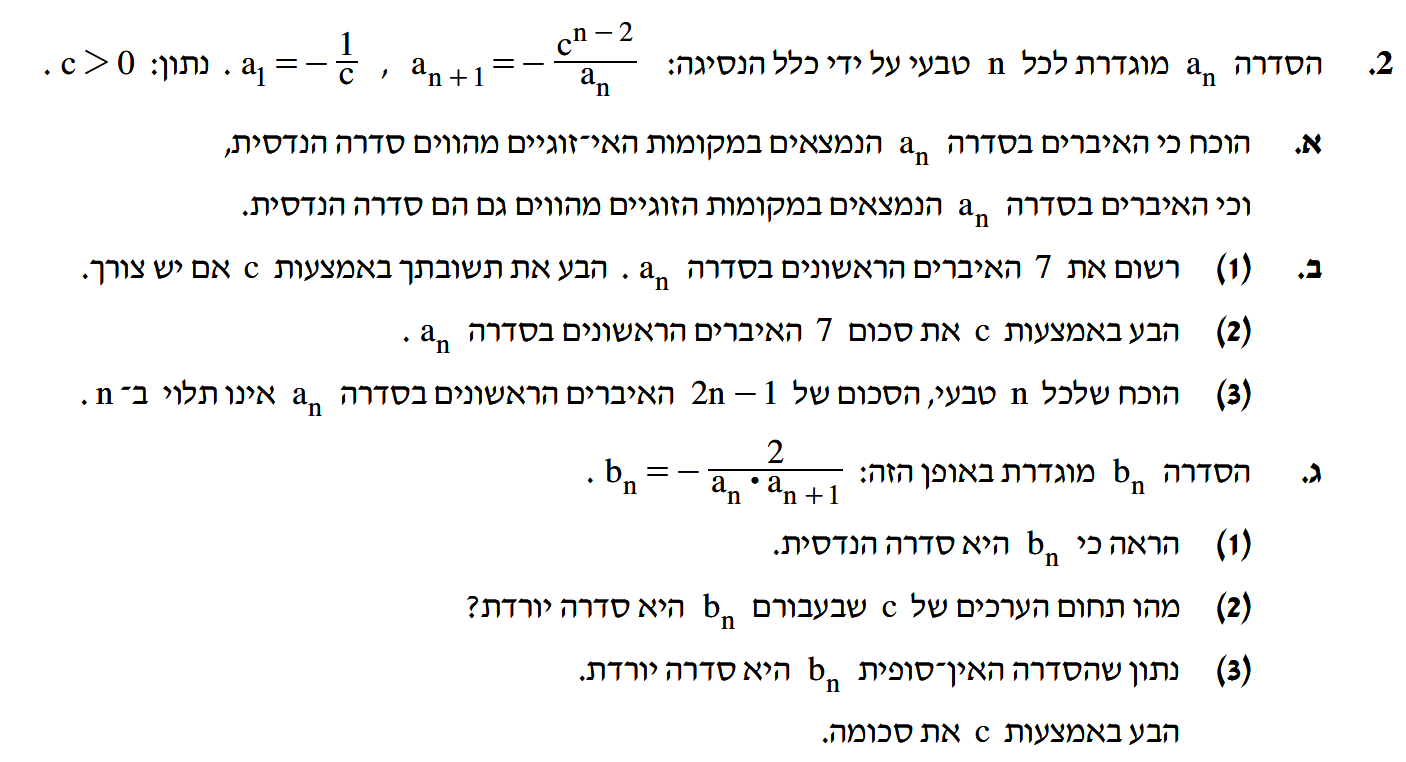
\includegraphics[width=\textwidth]{summer-2018b-2}
\end{center}
\vspace{-1ex}

\textbf{סעיף א}

כדי להוכיח שסדרה המוגדרת על ידי כלל נסיגה היא הנדסית, לא כדאי לחשב מנה של שני איברים עוקבים, כי איברים לא יצטמצמו. במקום זה, יש להציב את כלל הנסיגה כדי לקבל ערך של איבר כתלות של איבר אחר:
\[
a_{n+1} = -\frac{c^{n-2}}{a_n} = -\frac{c^{n-2}}{\displaystyle -\frac{c^{n-3}}{a_{n-1}}} = ca_{n-1}\,.
\]
המנה
$a_{n+1}/a_{n-1}=c$
קבועה ולא תלוי ב-%
$n$.
ההוכחה נכונה עבור כל זוג של איברים שיש הפרש של שניים במקומות שלהם בסדרה, ולכן ההוכחה נכונה גם עבור זוגות של מספרים זוגיים וגם עבור זוגות של מספרים א-זוגיים.

\smallskip

\textbf{סעיף ב}
$(1)$

הסדרות של הזוגיים והאי-זוגיים הן סדרות הנדסיות
\textbf{נפרדות}
ויש לחשב את האיברים בנפרד:

\vspace{-2ex}

\[
\erh{12pt}
\begin{array}{l}
a_1=-\displaystyle\frac{1}{c},\;\;a_3=ca_1=-1,\;\;a_5=ca_3=-c,\;\;a_7=ca_5=-c^2\\
a_2=\displaystyle
-\frac{c^{1-2}}{a_1}=
-\frac{c^{-1}}{-\frac{1}{c}}=1,\;\;a_4=ca_2=c,\;\;a_6=ca_4=c^2\,.
\end{array}
\]
שבעת האיברים הראשונים של הסדרה הם:
\[
-\frac{1}{c}\,,1\,, -1\,, c\,, -c\,, c^2\,, -c^2\,.
\]

\np

\textbf{סעיף ב}
$(2)$

כאשר מסכמים את האיברים הם מצטמצמים פרט לאיבר הראשון, ולכן
$S_7=-\frac{1}{c}$.

\smallskip

\textbf{סעיף ב}
$(3)$

כאשר יש מספר אי-זוגי של איברים המתחילים ממקום אי-זוגי, מספר האיברים האי-זוגיים גדול באחד ממספר האיברים הזוגיים. נבדוק דוגמה:
\[
a_1\,,a_2\,,a_3\,,a_4\,,a_5\,,a_6\,,a_7\,,a_8\,,a_9\,.
\]
מספר האיברים הוא
$9$,
מהם
$5$
אי-זוגיים ו-%
$4$
זוגיים.

נצטרך לסכם את זוגיים והאי-זוגיים בנפרד, כי הסדרה המקורית אינה הנדסית. עבור שתי התת-סדרות, המנה הוא 
$c$,
אבל האיבר הראשון שונה 
$-\frac{1}{c}, 1$:
\[
S_{\mathit{odd}}+S_{\mathit{even}}=-\frac{1}{c}\frac{c^n-1}{c-1}+ 1\cdot\frac{c^{n-1}-1}{c-1}=
%\frac{-c^{n-1}+c^{-1} + c^{n-1}-1}{c-1}=
-\frac{1}{c}\,,
\]
לא תלוי ב-%
$n$.

\smallskip

\textbf{סעיף ג}
$(1)$

כאן הסדרה נתונה על ידי נוסחה ולא כלל נסיגה ולכן ניתן לחשב ישירות את המנה:
\[
\frac{b_{n+1}}{b_n} = \frac{\displaystyle\frac{2}{a_{n+1}a_{n+2}}}{\displaystyle\frac{2}{a_{n}a_{n+1}}}= \frac{\displaystyle \frac{1}{a_{n+2}}}{\displaystyle \frac{1}{a_{n}}} =  \frac{1}{\displaystyle\frac{a_{n+2}}{a_n}} = \frac{1}{c}\,.
\]
\textbf{סעיף ג}
$(2)$

סדרה יורדת אם
$0<q=\displaystyle\frac{1}{c} < 1$.
נתון
$c>0$,
ולכן הסדרה יורדת אם
$c>1$.

\smallskip

\textbf{סעיף ג}
$(3)$

עבור סדרה הנדסית יורדת:
\erh{14pt}
\begin{equationarray*}{rcl}
S_b&=&\displaystyle\frac{b_1}{1-(1/c)}\\
&=&\frac{-2}{a_1\cdot a_{2}}\cdot \frac{c}{c-1}\\
&=&\frac{-2}{\displaystyle-\frac{1}{c}\cdot  1}\cdot \frac{c}{c-1}\\
&=&\frac{2c^2}{c-1}\,.
\end{equationarray*}

%%%%%%%%%%%%%%%%%%%%%%%%%%%%%%%%%%%%%%%%%%%%%%%%%%%%%%%%%%%%%%%%%%%
\np
\section{קיץ תשע"ח מועד א}

\begin{center}
\selectlanguage{english}
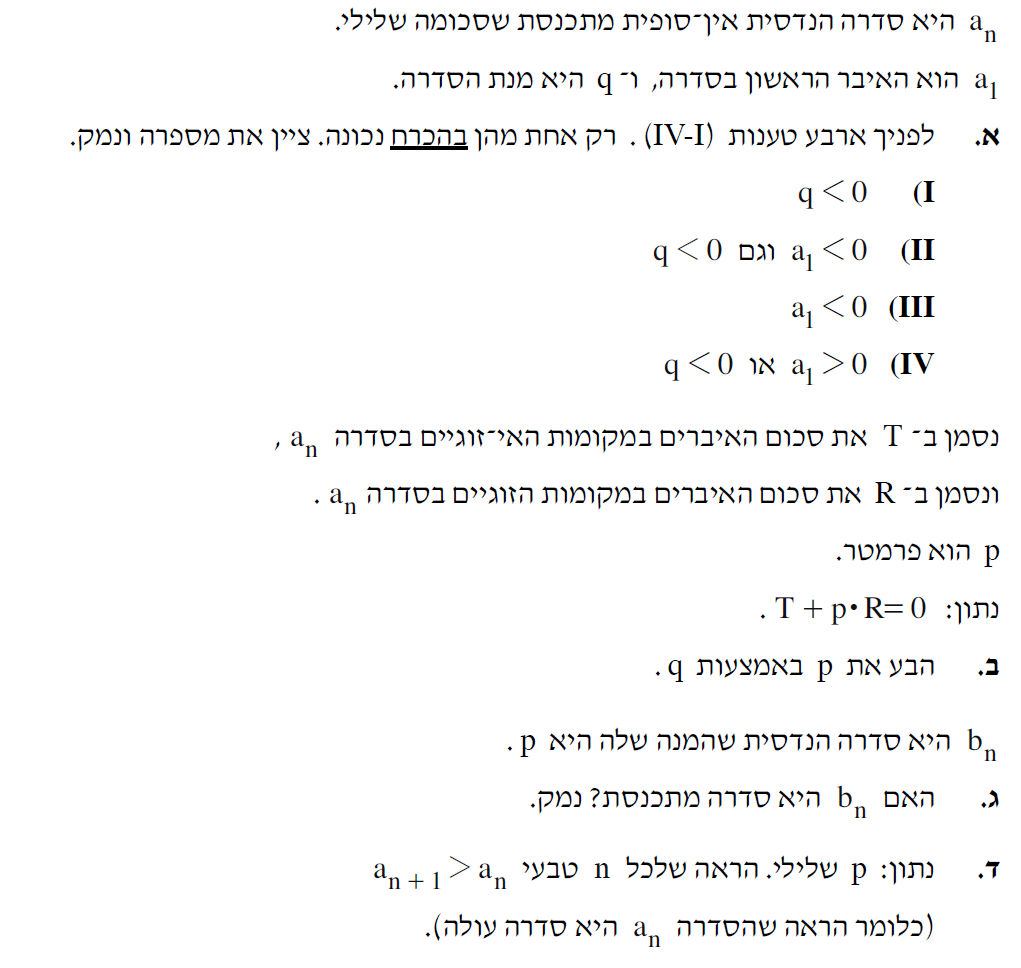
\includegraphics[width=.95\textwidth]{summer-2018a-2}
\end{center}

\textbf{סעיף א}

השאלה יפה כי היא דורשת חשיבה, לא חישובים! נבדוק את הטענות על סדרה מוכרת:
\[
1+ \frac{1}{2} + \frac{1}{4} + \frac{1}{8} + \cdots = 2\,.
\]
אם נהפוך את כל הסימנים למינוס, נקבל סדרה שסכומה שלילי:
\[
-1 - \frac{1}{2} - \frac{1}{4} - \frac{1}{8} - \cdots = -\left(1+ \frac{1}{2} + \frac{1}{4} + \frac{1}{8} + \cdots\right) = -2\,.
\]
ברור שהמנה עדיין חיובית:
\[
\frac{-2^{-(n+1)}}{-2^{-n}}=2^{-1}=\frac{1}{2}\,.
\]
לכן אפשר לפסול מייד תשובות 
\L{I, II, IV}
ונשאר רק תשובה
\L{III}.

\np

נעבור לסדרה כללית. סדרה הנדסית מתכנסת רק אם
$|q|<1$.
מהנוסחה עבור הסכום:
\[
S = \frac{a_1}{1-q} <0\,,
\]
ניתן לראות ש-% 
$a_1$
שלילי כי המכנה חיובי
$0 < 1-q < 2$.

\smallskip

\textbf{סעיף ב}

כאן מדובר בתת-סדרות של סדרה הנדסית, ועוד תת-סדרות שאיבריהן במקום קבוע אחד מהשני )הפרש של שני מקומות: זוגי לזוגי או אי-זוגי לאי-זוגי(. לכן, המנה של כל אחת מהסדרות היא
$q^2$,
והסכומים הם:
\[
T = \frac{a_1}{1-q^2},\quad\quad R = \frac{a_1q}{1-q^2}\,.
\]
מהמשוואה הנתונה
$T+pR=0$,
נקבל
$\quad 1+pq=0\quad$
ו-%
$p=-\displaystyle\frac{1}{q}\quad$.

\smallskip

\textbf{סעיף ג}

הסדרה לא מתכנסת כי 
$|q|<1$
גורר
$|p|>1$.

\smallskip

\textbf{סעיף ד}

שימו לב שהשאלה שואלת על
\textbf{הסדרה המקורית}
$a_n$
ולא על 
$b_n$!
נתון ש-%
$p$
שלילי ולכן
$q=-\displaystyle\frac{1}{p}$
חיובי. נתון שהסדרה מתכנסת ולכן
$0<q<1$.
מצאנו בסעיף א ש-%
$a_1$
שלילי ולכן
$a_{n+1}>a_n$,
כי מכפלה של מספר שלילי
$x$
עם מספר חיובי פחות מ-%
$1$
מקטינה את הערך המוחלט
$|x|$
ומורידה את
$-|x|$.

נבדוק בדוגמה: אם 
$a_n=-6,q=\frac{1}{2}$,
אז:
\[
a_{n+1} = a_nq = -6\cdot \frac{1}{2} = -3 \;> \; -6 =a_n\,.
\]


%%%%%%%%%%%%%%%%%%%%%%%%%%%%%%%%%%%%%%%%%%%%%%%%%%%%%%%%%%%%%%%%%%%

\np
\section{חורף תשע"ח}

\begin{center}
\selectlanguage{english}
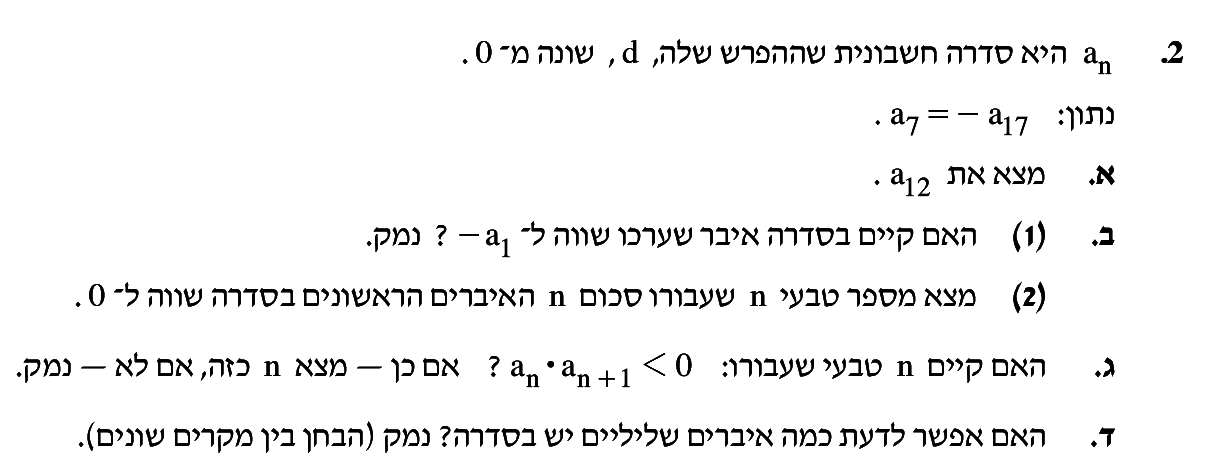
\includegraphics[width=.95\textwidth]{winter-2018-2}
\end{center}

\vspace{-1ex}

שאלה זו מתאפיין בהצבה של נוסחאות לאיברים מסויימים לתוך הנוסחאות הכלליות.

\smallskip

\textbf{סעיף א}

נציב 
$a_1+(n-1)d$
במשוואה
$a_7=-a_{17}$:
\[
\erh{2pt}
\begin{array}{l}
a_7=a_1+6d = -(a_1+16d)=-a_{17}\\
a_1+11d=0\\
a_{12}=a_1+11d=0\,.
\end{array}
\]
\textbf{סעיף ב}
$(1)$

נשווה את
$-a_1$
לנוסחה לאיבר כללי:
\[
-a_1 = a_n = a_1 + (n-1)d\,.
\]
נציב
$a_1=-11d$
שישבנו בסעיף א:
\[
-(-11d) = -11d + (n-1)d\,.
\]
$d$
מצטמצם ונקבל
$n=23$.

\smallskip

\textbf{סעיף ב}
$(2)$

נציב
$a_1=-11d$
 בנוסחה לסכום של סדרה חשבונית:
\[
\frac{n}{2}(2a_1+(n-1)d) = \frac{n}{2}(2\cdot -11d+(n-1)d) =\frac{dn}{2} (n-23)=0\,.
\]
נתון שההפרש 
$d$
שונה מאפס וש-%
$n$
מספר טבעי ולכן חיובי, כך שהביטוי מתאפס רק עבור
$n=23$.

\np

\textbf{סעיף ג}

אם איבר חיובי וההפרש חיובי, המכפלה של שני איברים עוקבים היא חיובית, וכך גם אם שניהם שליליים. האפשרות היחידה לקבל מכפלה שלילית היא איבר שלילי והפרש חיובי או איבר חיובי והפרש שלילי:
\[
\erh{2pt}
\begin{array}{l}
a_k<0,\; a_{k+1}>0\\
a_k>0,\; a_{k+1}<0\,.
\end{array}
\]
אבל ידוע שאחד האיברים בסדרה 
$(a_{12})$
הוא אפס:
\[
\erh{2pt}
\begin{array}{l}
a_k<0,\; a_{k+1}=0,\; a_{k+2}>0\\
a_k>0,\; a_{k+1}=0,\; a_{k+2}<0\,,
\end{array}
\]
ולכן המכפלה של זוג איברים עוקבים חייבת להיות חיובית או אפס.

\smallskip

\textbf{סעיף ד}

נרשום את הסדרה לפי מה שיודע לנו ש-%
$a_{12}=0$:
\[
a_1,\; a_2,\; \ldots,\; a_{11},\; 0,\; -a_{11},\; \ldots,\; -a_2,\; -a_1,\; \ldots\,.
\]
או ש-%
$11$
האיברים הראשונים שליליים אם ההפרש חיובי, או כל האיברים לאחר האיבר
$a_{12}=0$
שליליים אם ההפרש שלילי.



%%%%%%%%%%%%%%%%%%%%%%%%%%%%%%%%%%%%%%%%%%%%%%%%%%%%%%%%%%%%%%%%%%%
\np
\section{קיץ תשע"ז מועד ב}

\begin{center}
\selectlanguage{english}
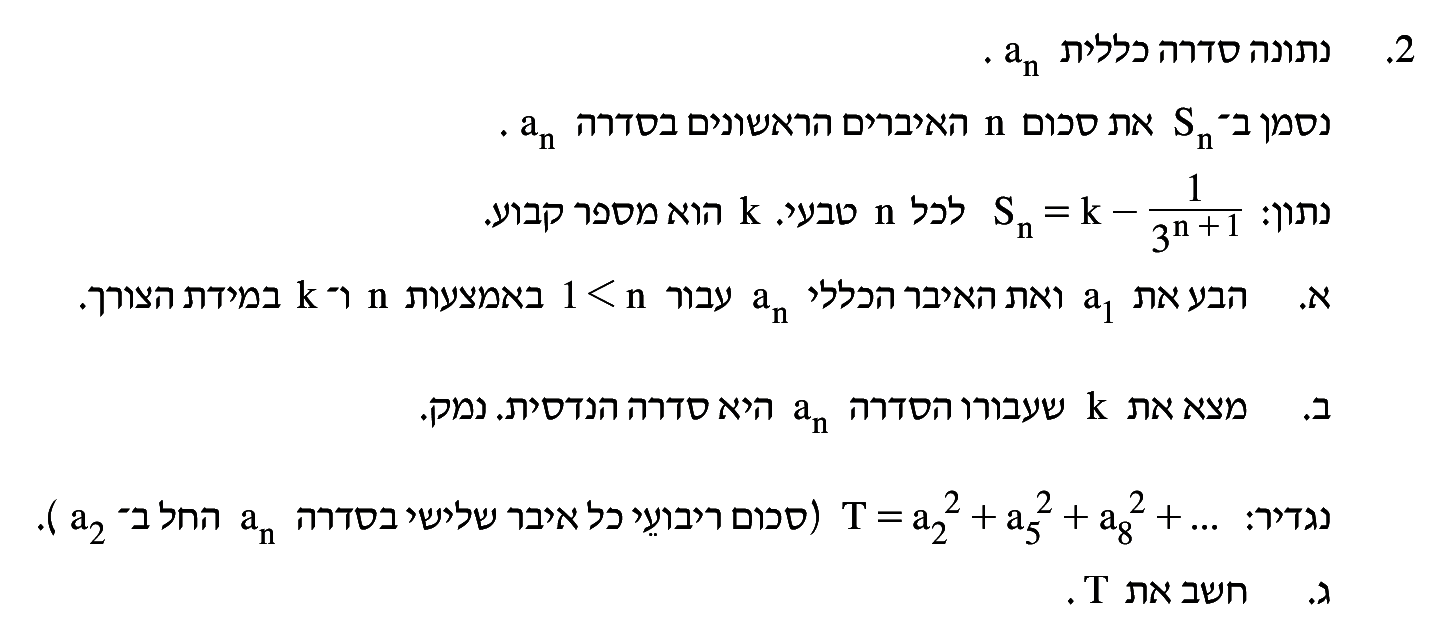
\includegraphics[width=.95\textwidth]{summer-2017b-2}
\end{center}

שאלה זו שונה משאלות אחרות כי נתון ביטוי עבור
\textbf{הסכומים}
ולא עבור האיברים בסדרה.

\smallskip

\textbf{סעיף א}

ניתן לחשב את האיברים על ידי שימוש בנוסחה עבור
$S_n$.
האיבר הראשון מתקבל ישירות מהנוסחה:
\[
a_1=S_1=k-\frac{1}{3^{1+1}}=k-\frac{1}{9}\,,
\]
והאיבר הכללי מתקבל על ידי ההפרש בין הנוסחאות לסכומים עוקבים:
\[
a_n=S_{n}-S_{n-1}=\left(k-\frac{1}{3^{n+1}}\right)-\left(k-\frac{1}{3^{n}}\right)=\frac{2}{3^{n+1}}\,.
\]
\textbf{סעיף ב}

המנה
$q=\displaystyle\frac{a_{n+1}}{a_{n}}=\frac{1}{3}$
לא תלויה ב-%
$k$.
במבט ראשון נראה שהתשובה היא שהסדרה היא הנדסית עבור כל ערך של
$k$,
אולם זו
\textbf{טעות}.
המנה המתקבלת מ-%
$\displaystyle\frac{a_2}{a_1}$
חייבת להיות
\textbf{שווה}
למנה המתקבלת מהמקרה הכללי
$\displaystyle\frac{a_{n+1}}{a_{n}}$.
נחשב:
\[
\frac{a_2}{a_1}=\frac{\displaystyle\frac{2}{3^3}}{\displaystyle k-\frac{1}{9}} =  \frac{2}{3(9k-1)} =\frac{a_{n+1}}{a_n}=\frac{1}{3}\,.
\]
הפתרון היחיד הוא
$\displaystyle k=\frac{1}{3}$.

עבור הסעיף הבא נצטרך את האיבר הראשון:
\[
\displaystyle \frac{1}{3}-\frac{1}{9}=\frac{2}{9}\,,
\]

\np

\textbf{סעיף ג}

האיבר הראשון בסדרה החדשה הוא:
\[
a'_1 = a_2^2=\left(a_1q\right)^2=\left(\frac{2}{9}\cdot\frac{1}{3}\right)^2=\frac{4}{729}\,,
\]
הסדרה החדשה היא הנדסית:
\[
\left(\frac{a_{3(k+1)-1}}{a_{3k-1}}\right)^2 =  \left(\frac{qa_{3k+1}}{a_{3k-1}}\right)^2=\left(\frac{q^2a_{3k}}{a_{3k-1}}\right)^2=\left(\frac{q^3a_{3k-1}}{a_{3k-1}}\right)^2=q^6=\left(\frac{1}{3}\right)^6=\frac{1}{729}\,.
\]
הסכום מתקבל מהנוסחה לסדרה הנדסית אינסופית עבור
$a', q'$:
\[
S'=\frac{a'_1}{1-q'}=
\frac{\displaystyle\frac{4}{729}}{1-\displaystyle\frac{1}{729}}= \frac{1}{182}\,.
\]

%%%%%%%%%%%%%%%%%%%%%%%%%%%%%%%%%%%%%%%%%%%%%%%%%%%%%%%%%%%%%%%%%%%
\np
\section{קיץ תשע"ז מועד א}

\begin{center}
\selectlanguage{english}
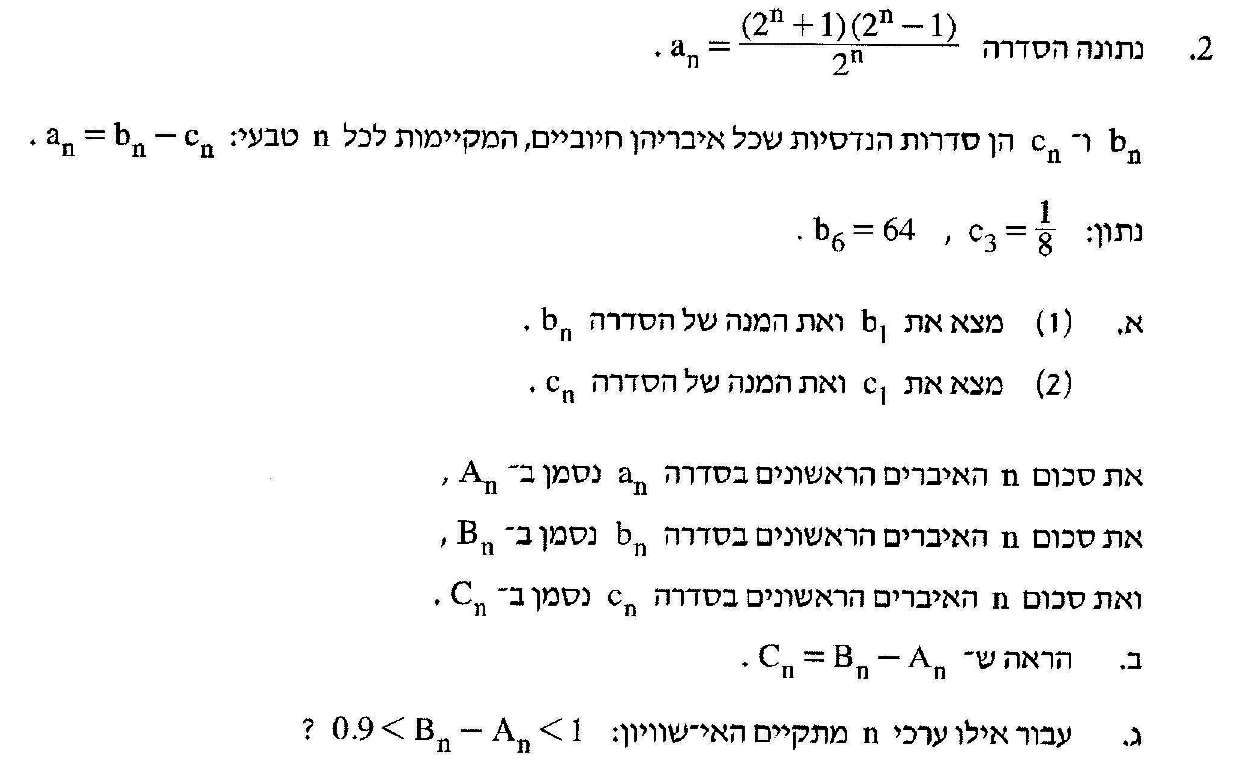
\includegraphics[width=.95\textwidth]{summer-2017a-2}
\end{center}
הנוסחה ל-%
$a_n$
אינה כלל נסיגה כי איברים של הסדרה לא מופיעים בצד הימני של המשוואה. נתון שהסדרות 
$b_n,c_n$
הנדסיות אך לא נתון אם הסדרה המקורית
$a_n$
הנדסית או לא.

\textbf{סעיף א}
$(1,2)$

נתון ש-%
$a_n=b_n-c_n$,
לכן כדי לקבל ערך של איבר בסדרה
$b_n$,
נצטרך לחשב את הערכים
$a_n,c_n$,
ובאופן דומה עבור איברים בסדרה
$c_n$.
נתון שני ערכים
$b_6,c_3$
וקל לחשב איברים ב-%
$a_n$
כי הם נתונים כפונקציה של 
$n$ 
בלבד:
\[
\erh{18pt}
\begin{array}{l@{\hspace{3em}}l}
\displaystyle a_3=\frac{(2^3+1)(2^3-1)}{2^3}=\frac{63}{8}&\displaystyle a_6=\frac{(2^6+1)(2^6-1)}{2^6}= \frac{65\cdot 63}{64}\\
\displaystyle b_3=a_3+c_3=\frac{63}{8}+\frac{1}{8}=8 &\displaystyle  c_6=b_6-a_6=64-\frac{65\cdot 63}{64}=\frac{1}{64}\,.
\end{array}
\]
כדי לחשב את מנה של
$b_n$
והמנה של
$c_n$
נשתמש בעבודה שהן סדרות הנדסיות וכדי לקבל את האיבר הששי מהאיבר השלישי יש להכפיל במנה לחזקת שלוש:
\vspace{-1ex}
\[
\erh{22pt}
\begin{array}{l@{\hspace{2em}}l@{\hspace{5em}}l@{\hspace{2em}}l}
b_6=b_3q_b^3 & \displaystyle q_b=\sqrt[3]{\frac{b_6}{b_3}}=\sqrt[3]{8}=2& b_3=b_1 q_b^2 & \displaystyle b_1=\frac{b_3}{q_b^2}=\frac{8}{4}=2\\
c_6=c_3q_c^3 & \displaystyle q_c=\sqrt[3]{\frac{c_6}{c_3}} =\sqrt[3]{\frac{1}{8}} = \frac{1}{2}& c_3=c_1 q_c^2 & \displaystyle c_1=\frac{c_3}{q_c^2}=\frac{1/8}{1/4}=\frac{1}{2}
\end{array}
\]

\np

\textbf{סעיף ב}

הטיעון נובע מחוקי הקיבוץ והחילוף של מספרים שלמים:
\begin{eqnarray*}
C_n &=& (b_1-a_1) + (b_2 - a_2) + \cdots + (b_n-a_n)\\
&=&(b_1 + b_2 + \cdots + b_n) - (a_1 + a_2 + \cdots + a_n)\\
&=& B_n - A_n\,.
\end{eqnarray*}
\textbf{סעיף ג}

הוכחנו ש-%
$C_n=B_n-A_n$,
ונתונה שהסדרה 
$c_n$
הנדסית. מסעיף א
$\displaystyle q_c=\frac{1}{2},\,c_1=\frac{1}{2}$,
ולכן:
\[
C_n = \frac{1}{2}\cdot\frac{\displaystyle\left(\left(\frac{1}{2}\right)^n-1\right)}{\displaystyle\left(\frac{1}{2}-1\right)}=1-2^{-n}\,.
\]
בדיקה במחשבון מראה ש:
%\vspace{-2ex}
\[
\erh{8pt}
\begin{array}{l}
0.9 \not< 1-2^{-3}=0.875<1\\
0.9 < 1-2^{-4}=0.938 < 1\,.
\end{array}
\]

לא לעצור כאן! השאלה מבקשת את
\textbf{כל הערכים}
של
$n$
המקיימים את האי-שוויון, ולכן התשובה המליאה היא כל מספר גדול או שווה ל-%
$4$,
כי כאשר 
$n$
גדל מעל ל-%
$4$,
הערך של 
$1-2^{-n}$
עולה )ולכן גדול מ-%
$0.9$(
אבל תמיד פחות מ-%
$1$.

%%%%%%%%%%%%%%%%%%%%%%%%%%%%%%%%%%%%%%%%%%%%%%%%%%%%%%%%%%%%%%%%%%%
\np
\section{חורף תשע"ז}

\begin{center}
\selectlanguage{english}
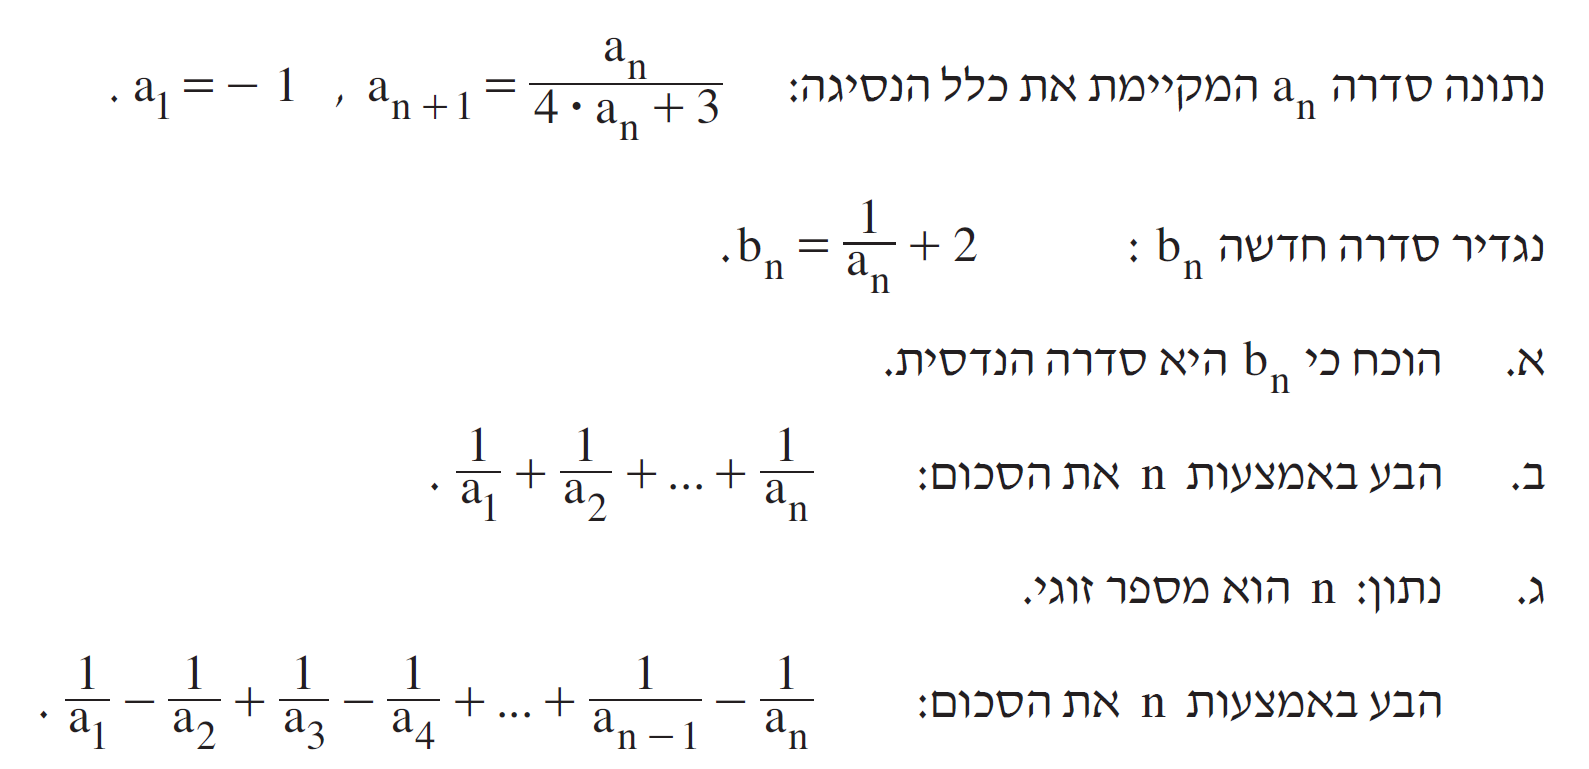
\includegraphics[width=.9\textwidth]{winter-2017-2}
\end{center}

\vspace{-2ex}

\textbf{סעיף א}

נחשב את המנה על ידי הצבה עבור 
$b_n$
לפי ההגדרה, ואחר כך הצבה עבור 
$a_{n+1}$
לפי כלל הנסיגה. נקבל מנה קבועה ולכן הסדרה הנדסית:
\[
\frac{b_{n+1}}{b_n} = \frac{\displaystyle\frac{1}{a_{n+1}}+2}{\displaystyle\frac{1}{a_{n}}+2}= \frac{\displaystyle\frac{4a_n+3}{a_n}+2}{\displaystyle\frac{1}{a_{n}}+2}=\frac{3(2a_n+1)}{2a_n+1}=3\,.
\]
\vspace{-3ex}

\textbf{סעיף ב}

לא נתון שהסדרה $a_n$ הנדסית, אבל בסעיף א הוכחנו שהסדרה  
$b_n$
הנדסית, ולכן ניתן לבטא את סכום הסדרה
$\displaystyle\frac{1}{a_n}$
כסכום של הסדרה
$b_n$
על ידי ההצבה 
$\displaystyle\frac{1}{a_i} = b_i - 2$:
\[
\frac{1}{a_1} + \cdots + \frac{1}{a_n}=(b_1-2) + \cdots + (b_n-2)=b_1+\cdots+b_n- 2n\,.
\]
נתון ש
$a_1=-1$,
כך ש-%
$b_1=\displaystyle\frac{1}{a_1}+2=1$
ובסעיף א חישבנו 
$q_b=3$.
סכום הסדרה של 
$\displaystyle \frac{1}{a_n}$
הוא:
\[
b_1+\cdots+b_n- 2n=\frac{1(3^n-1)}{3-1} - 2n = \frac{3^n - 4n -1}{2}\,.
\]
\textbf{סעיף ג}

לפי ההגדרה של 
$b_n$
נוכל לבטא את הסכום כך:
\[
(b_1 - 2) - (b_2 - 2) + \cdots + (b_{n-1} - 2) - (b_n - 2)\,.
\]
נתון שמספר האיברים זוגי ולכן סכום הקבועים מתאפס. המנה של הסדרה היא
$-3$
והסכום הוא:
\[
b_1-b_2+\cdots+b_{n-1}-b_n=\frac{1((-3)^n-1)}{-3-1}=\frac{(-3)^n-1}{-4}=\frac{1-3^n}{4}\,,
\]
כי מספר האיברים זוגי ולכן
$(-3)^n=3^n$.


%%%%%%%%%%%%%%%%%%%%%%%%%%%%%%%%%%%%%%%%%%%%%%%%%%%%%%%%%%%%%%%%%%%

\np
\section{קיץ תשע"ו מועד ב}

\begin{center}
\selectlanguage{english}
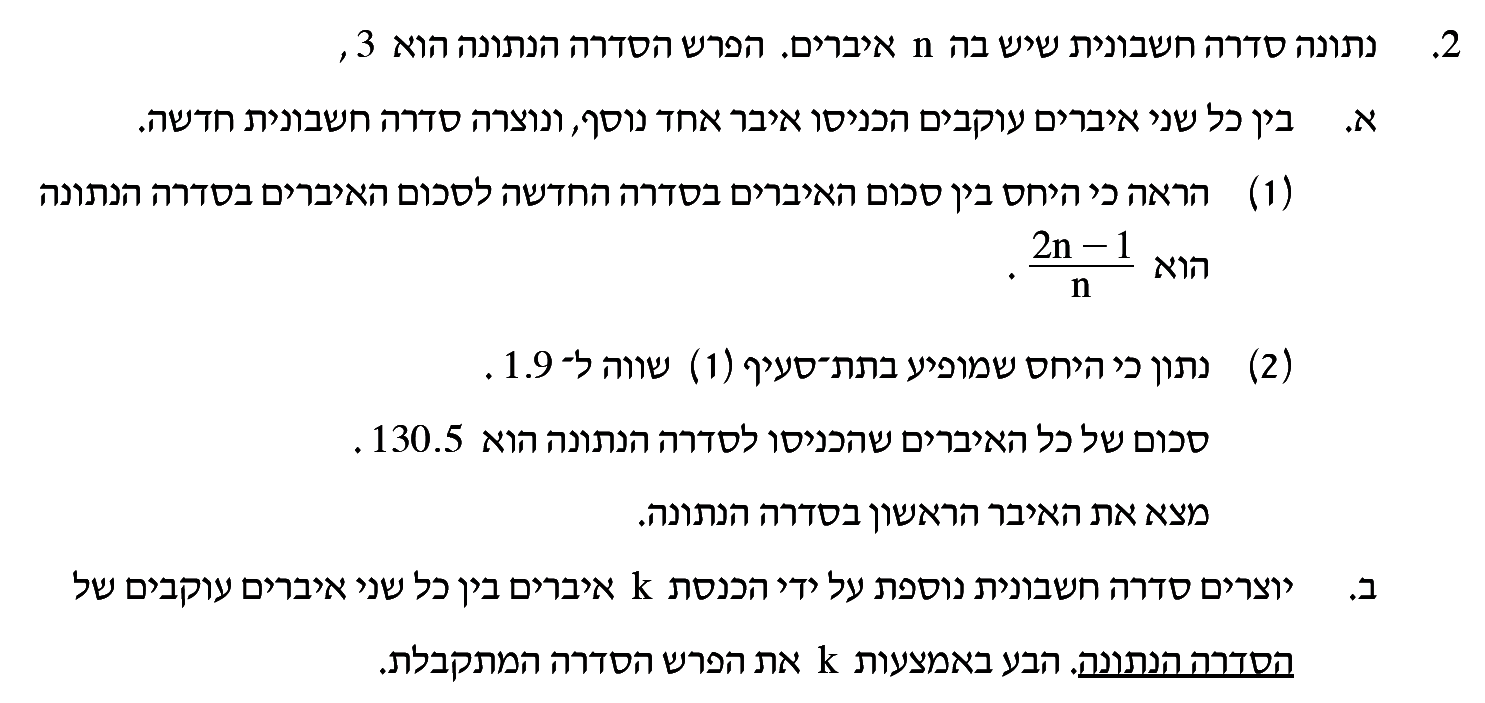
\includegraphics[width=.95\textwidth]{summer-2016b-2}
\end{center}
\vspace{-1ex}

\textbf{סעיף א}
$(1)$

מספר האיברים החדשים הוא
$n-1$,
כפי שרואים אם רושמים את הסדרה:
\[
a_1,\; a'_1,\; a_2,\; a'_2,\; \ldots,\; a_{n-1},\; a'_{n-1},\; a_n\,.
\]
נתון שהסדרה החדשה גם היא חשבונית. הפרש הסדרה אינו מספר שלם אלא
$1.5$!
אז מה? נחשב את היחס בין סכומי הסדרות, כאשר האיבר
$a_1$
מצטמצם:
\[
\frac{S_{\mathit{new}}}{S_{\mathit{old}}}= \frac{\displaystyle\frac{2n-1}{2}(2a_1+1.5(2n-1-1))}{\displaystyle\frac{n}{2}(2a_1+3(n-1))}=\frac{\displaystyle\frac{2n-1}{2}(2a_1+3(n-1))}{\displaystyle\frac{n}{2}(2a_1+3(n-1))}=\frac{2n-1}{n}\,.
\]
\textbf{סעיף א}
$(2)$

מ-%
$\displaystyle\frac{2n-1}{n}=1.9$
נקבל
$n=10$. 
אם הסדרה הנתונה חשבונית וגם הסדרה החדשה חשבונית, סדרת האיברים החדשים היא חשבונית עם אותו הפרש כמו בסדרה המקורית, 
$3$.
%
%נתון שהסדרה החדשה חשבונית ולכן גם סדרת האיברים החדשים חשבונית:
%\[
%a'_{i+1}-a'_{i}=a'_{i+1}-(a_{i+1}-a_{i+1})-a'_i=(a'_{i+1}-a_{i+1})+(a_{i+1}-a'_i)=\frac{d}{2}+\frac{d}{2}=3\,.
%\]
האיבר הראשון של האיברים החדשים הוא
$a'_1=a_1+1.5$,
ונתון סכום האיברים החדשים:
\[
\frac{10-1}{2}(2(a_1+1.5)+((10-1)-1)\cdot 3) = 130.5\,,
\]
והפתרון הוא
$a_1=1$.

\textbf{סעיף ב}

נתון שהסדרה המתקבלת לאחר הכנסת
$k$
איברים חדשים בין איברים סמוכים של הסדרה הנתונה:
\[
a_i,\; b_1,\; b_2,\; \ldots,\; b_k,\; a_{i+1}
\]
היא חשבונית. ההפרשים בין האיברים החדשים חייבים להיות שווים וסכומם שווה להפרש של הסדרה הנתונה שהוא
$3$.
יש
$k+1$
הפרשים שערכם
$\displaystyle\frac{3}{k+1}$.

%%%%%%%%%%%%%%%%%%%%%%%%%%%%%%%%%%%%%%%%%%%%%%%%%%%%%%%%%%%%%%%%%%%

\np
\section{קיץ תשע"ו מועד א}

\begin{center}
\selectlanguage{english}
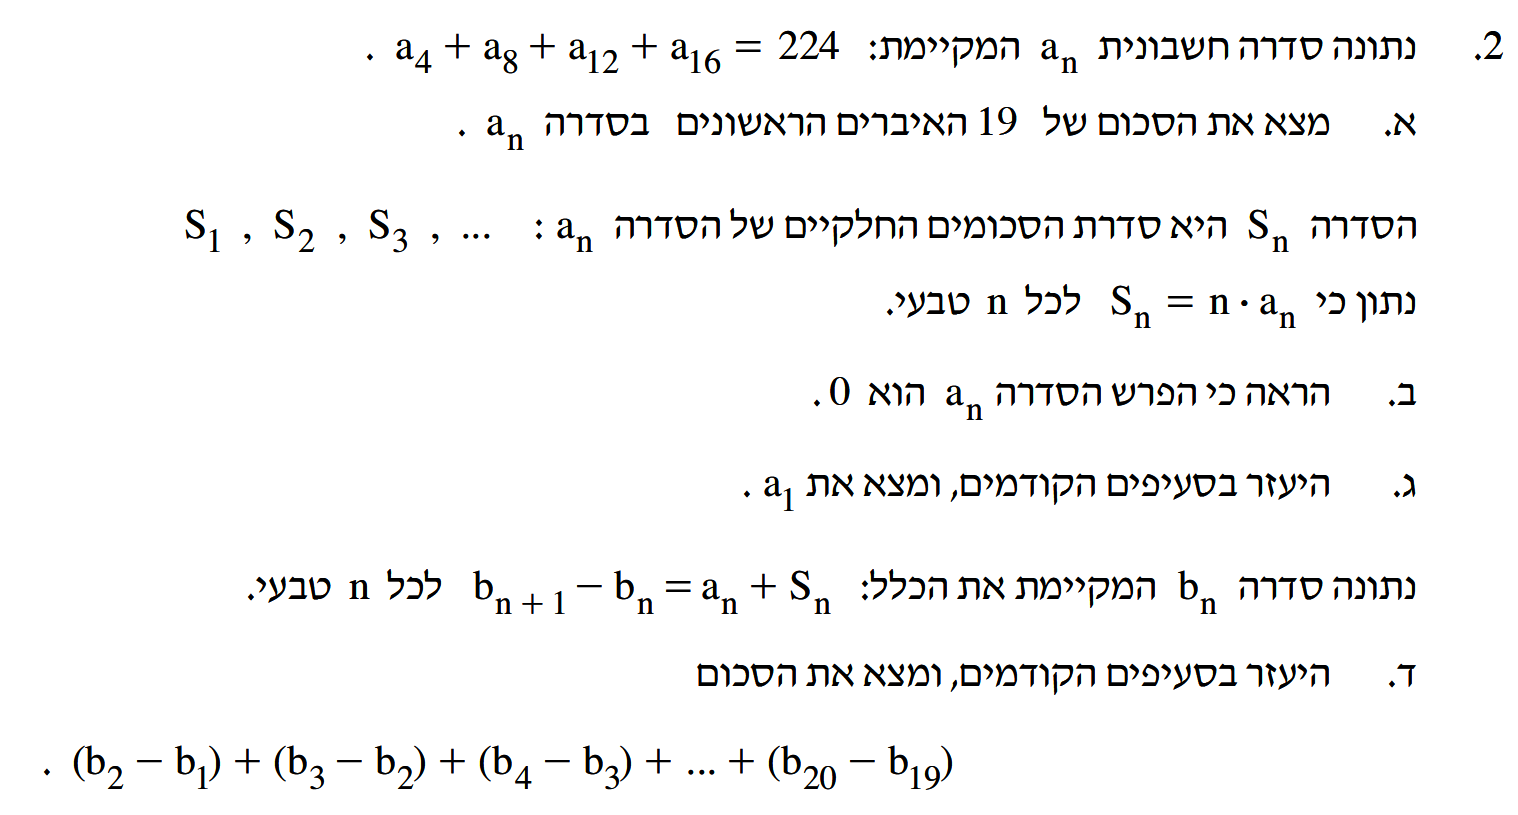
\includegraphics[width=.95\textwidth]{summer-2016a-2}
\end{center}
\vspace{-4ex}

\textbf{סעיף א}

האיברים
$a_4,a_8,a_{12},a_{16}$
מהווים סדרה חשבועית עם הפרש
$d^4$.
נתון הסכום של הסדרה:
\begin{eqnarray*}
(a_1+3d)+(a_1+7d)+(a_1+11d)+(a_1+15d)&=&224\\
a_1+9d&=&56\,.
\end{eqnarray*}
יש לנו משוואה אחת עם שני נעלמים. לא נתייאש וננסה בכל זאת לחשב את הסכום
$S_{19}$:
\[
S_{19}=\frac{19}{2}(2a_1+18d) = 19(a_1+9d)=19\cdot 56 = 1064\,.
\]
\vspace{-1ex}
\textbf{סעיף ב}

נשווה את המשוואה הנתונה
$S_n=n\cdot a_n$
לנוסחה עבור סכום של סדרה חשבונית:
\erh{10pt}
\begin{equationarray*}{rcl}
n\cdot a_n &=& \frac{n}{2}(2a_1+(n-1)d)\\
n(a_1+(n-1)d) &=&\frac{n}{2}(2a_1+(n-1)d)\,.
\end{equationarray*}
נפשט את המשוואה ונקבל 
$d=d/2$
שהפתרון היחיד שלה הוא
$d=0$.

\textbf{סעיף ג}

נציב
$0$
עבור 
$d$:
$a_1+9d=a_1+0=56$.

\textbf{סעיף ד}

במבט ראשון נראה שכדאי לצמצם את סכום הסדרה  ל-%
$b_{20}-b_1$,
אבל זה מבוי סתום כי אין לנו דרך לחשב את איברי הסדרה
$b_n$.
במקום זה נחשב את 
$(b_{i+1}-b_i)$
וניעזר במשוואה הנתונה:
\[
b_{i+1}-b_i=a_i+S_i=(a_1+(i-1)\cdot 0)+\frac{i}{2}(2a_1+(i-1)\cdot 0)=a_1(1+i)\,.
\]
הסכום הוא:
\[
a_1(2+3+\cdots+20)=56\cdot\frac{19}{2}(2\cdot 2 + (19-1)\cdot 1)=11704\,.
\]

%%%%%%%%%%%%%%%%%%%%%%%%%%%%%%%%%%%%%%%%%%%%%%%%%%%%%%%%%%%%%%%%%%%
\np
\section{חורף תשע"ו}

\begin{center}
\selectlanguage{english}
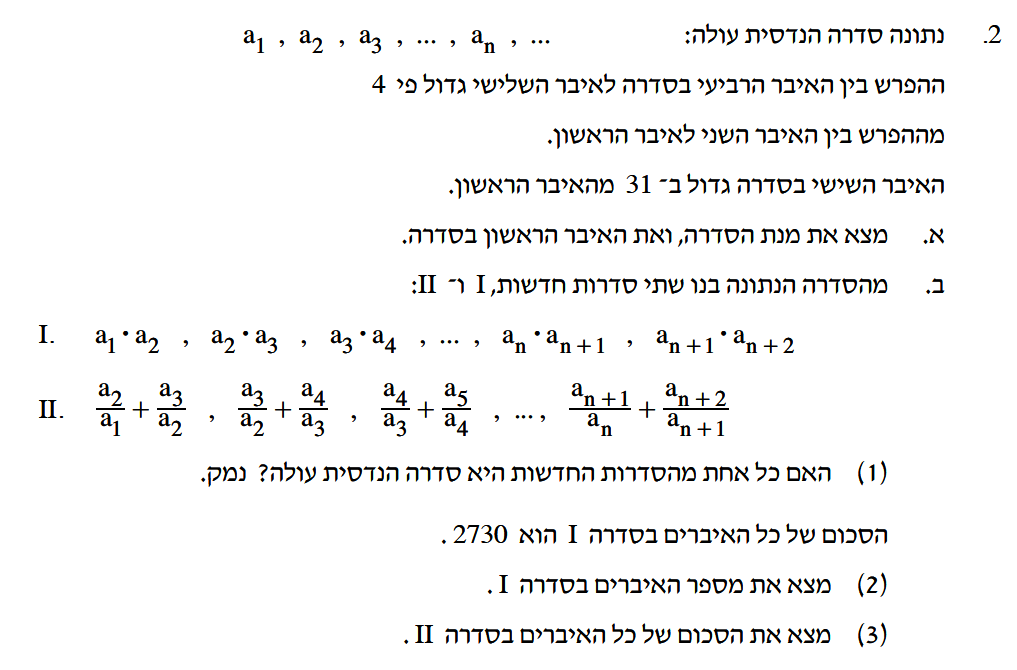
\includegraphics[width=.95\textwidth]{winter-2016-2}
\end{center}

\vspace{-3ex}

\textbf{סעיף א}

נתון:
\[
(1)\, a_4-a_3 = 4 (a_2-a_1),\quad (2)\, a_6 - a_1 = 31\,.
\]
נציב
$a_n=a_1q^{n-1}$ 
עבור
$a_2, a_3, a_4$,
ב-%
$(1)$,
ונקבל שלוש תשובות
$q=1,q=2,q=-2$.\\
נתון שהסדרה 
\textbf{עולה}
ולכן
$q=2$.
נציב 
$a_1q^5=32 a_1$
עבור
$a_6$
ב-%
$(2)$,
ונקבל
$a_1=1$.

\textbf{סעיף ב} 
$(1)$

עבור סדרה I:
\[
q_I=\frac{a_{n+1}\cdot a_{n+2}}{a_n\cdot a_{n+1}}=\frac{a_{n+2}}{a_n}=\frac{a_n\,q^2}{a_n}=q^2=4\,,
\]
והסדרה היא סדרה הנדסית עולה. עבור סדרה II:
\[
q_{II}=\left(\frac{a_{n+1}}{a_n} + \frac{a_{n+2}}{a_{n+1}}\right) / \left(\frac{a_{n}}{a_{n-1}} + \frac{a_{n+1}}{a_{n}}\right)=\frac{q+q}{q+q}=1\,.
\]
הסדרה הנדסית אבל
\textbf{לא עולה}.

\textbf{סעיף ב}
$(2)$

מסכום הסדרה ניתן לחשב את מספר האיברים בסדרה:
\begin{eqnarray*}
a_1\cdot a_2 + \cdots + a_{n+1} \cdot a_{n+2} &=& 2730\\
(1\cdot 2)\cdot \frac{4^{n+1}-1}{4-1}&=&2730\\
4^{n+1}&=&4096\\
n&=&5\,.
\end{eqnarray*}

\np

\textbf{שימו לב!}
אמנם
$n=5$
אבל מספר האיברים בסדרה I הוא 
$n+1=6$:
\[
(1)\, a_1\cdot a_2,\;\; (2)\,a_2\cdot a_3,\;\;(3)\, a_3\cdot a_4,\;\; (4)\,a_4\cdot a_5,\;\; (5)\,a_5\cdot a_6,\;\; (6)\,a_6\cdot a_7 \;(= a_{n+1}\cdot a_{n+2})\,.
\]
\textbf{סעיף ב}
$(2)$

חישבנו
$q_{II}=1$.
נחשב את
$a_1^{II}$:
\[
a_1^{II}=\frac{a_{2}}{a_1} + \frac{a_{3}}{a_{2}}=\frac{2}{1}+\frac{4}{2}=4\,.
\]
\textbf{שימו לב!}
מספר האיברים בסדרה II הוא 
$5$:
\[
(1)\,\frac{a_2}{a_1}+\frac{a_3}{a_2},\;\;
(2)\,\frac{a_3}{a_2}+\frac{a_4}{a_3},\;\;
(3)\,\frac{a_4}{a_3}+\frac{a_5}{a_4},\;\;
(4)\,\frac{a_5}{a_4}+\frac{a_6}{a_5},\;\;
(5)\,\frac{a_6}{a_5}+\frac{a_7}{a_6} \left(= \frac{a_{n+1}}{a_n}+\frac{a_{n+2}}{a_{n+1}}\right)\,.
\]
ולכן סכום האיברים הוא:
\[
a_1^{II}+a_1^{II}\cdot 1 + a_1^{II}\cdot 1^2 + \cdots + a_1^{II}\cdot 1^4 = 4\cdot 5=20\,.
\]


%%%%%%%%%%%%%%%%%%%%%%%%%%%%%%%%%%%%%%%%%%%%%%%%%%%%%%%%%%%%%%%%%%%
\np

\section{קיץ תשע"ה, מועד ב}

\begin{center}
\selectlanguage{english}
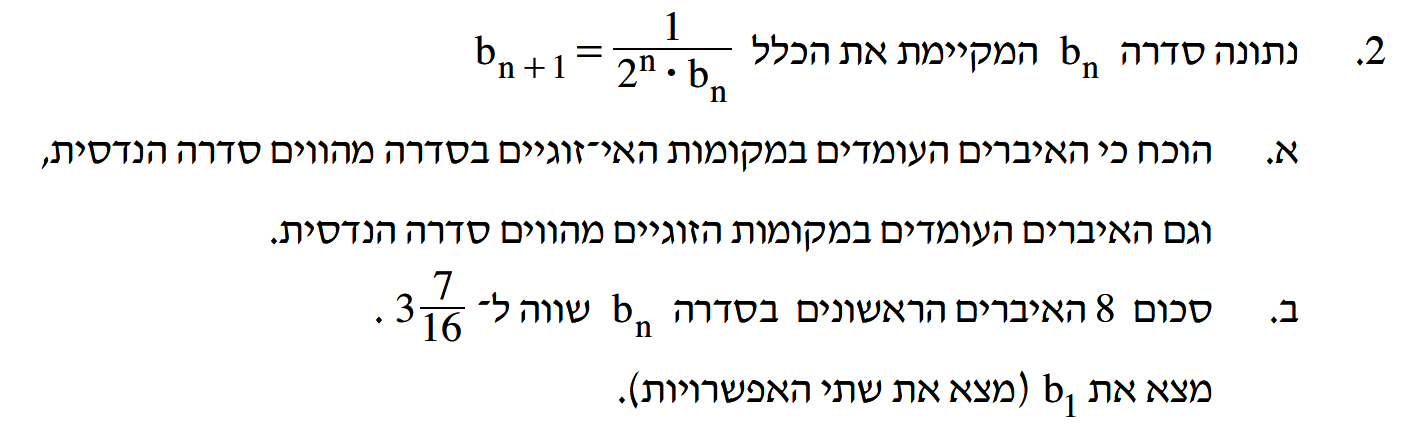
\includegraphics[width=.95\textwidth]{summer-2015b-2}
\end{center}
\vspace{-2ex}

\textbf{סעיף א}

החילוק של איברים במרחק שני מקומות אחד מהשני לא תלוי בזוגיות:
\[
\frac{b_{n+2}}{b_n} = \frac{1}{2^{n+1}b_{n+1}}\cdot\frac{1}{b_n}=\frac{1}{2^{n+1}\cdot\displaystyle\frac{1}{2^nb_n}{b_n}}= \frac{1}{2}\,.
\]
\textbf{סעיף ב}

 נחשב בנפרד את הסכום של ארבעת האיברים הזוגיים וארבעת האיברים האי-זוגיים:
\begin{eqnarray*}
S_{\mathit{odd}} &=& b_1+b_3+b_5+b_7=b_1\left(1 + \frac{1}{2} + \frac{1}{4} +\frac{1}{8}\right)=\frac{15}{8}b_1\\
S_{\mathit{even}} &=& b_2+b_4+b_6+b_8=b_2\left(1 + \frac{1}{2} + \frac{1}{4} +\frac{1}{8}\right)=\frac{15}{8}b_2=\frac{15}{8}\cdot\frac{1}{2^1b_1}\,.
\end{eqnarray*}
מ:
\[
S_{\mathit{odd}} + S_{\mathit{even}} =\frac{15}{8}\left(b_1+\frac{1}{2b_1}\right)= 3\frac{7}{16}=\frac{55}{16}\,.
\]
נקבל משוואה ריבועית 
$6b_1^2-11b_1+3=0$
שיש לה שני פתרונות 
$b_1=\frac{3}{2},\,\frac{1}{3}$.


%%%%%%%%%%%%%%%%%%%%%%%%%%%%%%%%%%%%%%%%%%%%%%%%%%%%%%%%%%%%%%%%%%%
\np

\section{חורף תשע"ו}

\begin{center}
\selectlanguage{english}
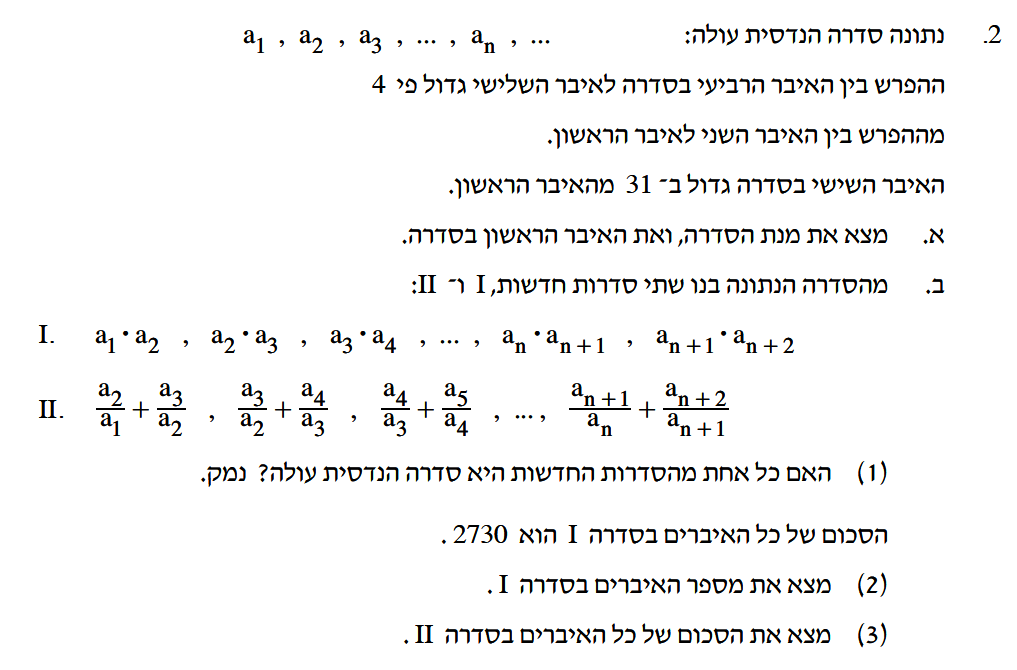
\includegraphics[width=.95\textwidth]{winter-2016-2}
\end{center}

\vspace{-4ex}

\textbf{סעיף א}

שימו לב ששואלים על
\textbf{ההפרשים}
של סדרה 
\textbf{הנדסית}.

המנתון הראשון:
\erh{2pt}
\begin{equationarray*}{rcl}
a_4-a_3 &=& 4 (a_2-a_1)\\
a_1q^3-a_1q^2 &=& 4(a_1q-a_1)\\
q^2(q-1)&=&4(q-1)\,.
\end{equationarray*}
\vspace{-5ex}

פתרון אחד של המשוואה הוא
$q=1$
אבל נתון שהסדרה עולה ולכן
$q\neq 1$.
אם 
$q\neq 1$,
נחלק ב-%
$q-1$
ונקבל
$q^2=4$.
כאשר המנה שלילי, הסימנים של איברי הסדרה מתחלפים, אז הפתרון היחיד הוא
$q=2$.

מהנתון השני:
\vspace{-2ex}
\erh{2pt}
\begin{equationarray*}{rcl}
a_6-a_1 &=& 31\\
a_1q^5-a_1&=& 31\\
32a_1-a_1&=&31\\
a_1&=&1\,.
\end{equationarray*}
\vspace{-6ex}

\textbf{סעיף ב} 
$(1)$

עבור סדרה I:
\[
q_I=\frac{a_{n+1}\cdot a_{n+2}}{a_n\cdot a_{n+1}}=\frac{a_{n+2}}{a_n}=\frac{a_n\,q^2}{a_n}=q^2=4\,,
\]
והסדרה היא סדרה הנדסית עולה.
\np

עבור סדרה II:
\[
q_{II}=\left(\frac{a_{n+1}}{a_n} + \frac{a_{n+2}}{a_{n+1}}\right) / \left(\frac{a_{n}}{a_{n-1}} + \frac{a_{n+1}}{a_{n}}\right)=\frac{q+q}{q+q}=1\,.
\]
הסדרה הנדסית אבל
\textbf{לא עולה}.

\smallskip

\textbf{סעיף ב}
$(2)$

מסכום הסדרה ניתן לחשב את מספר האיברים בסדרה:
\begin{eqnarray*}
a_1\cdot a_2 + \cdots + a_{n+1} \cdot a_{n+2} &=& 2730\\
(1\cdot 2)\cdot \frac{4^{n+1}-1}{4-1}&=&2730\\
4^{n+1}&=&4096\\
n&=&5\,.
\end{eqnarray*}
\begin{large}
\textbf{שימו לב!}
\end{large}
אמנם
$n=5$
אבל מספר האיברים בסדרה I הוא 
$n+1=6$:
\[
(1)\, a_1\cdot a_2,\;\; (2)\,a_2\cdot a_3,\;\;(3)\, a_3\cdot a_4,\;\; (4)\,a_4\cdot a_5,\;\; (5)\,a_5\cdot a_6,\;\; (6)\,a_6\cdot a_7 \;(= a_{n+1}\cdot a_{n+2})\,.
\]



\textbf{סעיף ב}
$(3)$

חישבנו
$q_{II}=1$.
נחשב את
$a_1^{II}$:
\[
a_1^{II}=\frac{a_{2}}{a_1} + \frac{a_{3}}{a_{2}}=\frac{2}{1}+\frac{4}{2}=4\,.
\]
\begin{large}
\textbf{שימו לב!}
\end{large}
מספר האיברים בסדרה II הוא 
$5$:
\[
(1)\,\frac{a_2}{a_1}+\frac{a_3}{a_2},\;\;
(2)\,\frac{a_3}{a_2}+\frac{a_4}{a_3},\;\;
(3)\,\frac{a_4}{a_3}+\frac{a_5}{a_4},\;\;
(4)\,\frac{a_5}{a_4}+\frac{a_6}{a_5},\;\;
(5)\,\frac{a_6}{a_5}+\frac{a_7}{a_6} \left(= \frac{a_{n+1}}{a_n}+\frac{a_{n+2}}{a_{n+1}}\right)\,.
\]

$q_{II}=1$
ולכן
\textbf{כל}
איברי הסדרה שווים ל-%
$a_1=4$.
הסכום הוא:
$4\cdot 5$.

%%%%%%%%%%%%%%%%%%%%%%%%%%%%%%%%%%%%%%%%%%%%%%%%%%%%%%%%%%%%%%%%%%%
\np
\section{קיץ תשע"ה מועד ב}

\begin{center}
\selectlanguage{english}
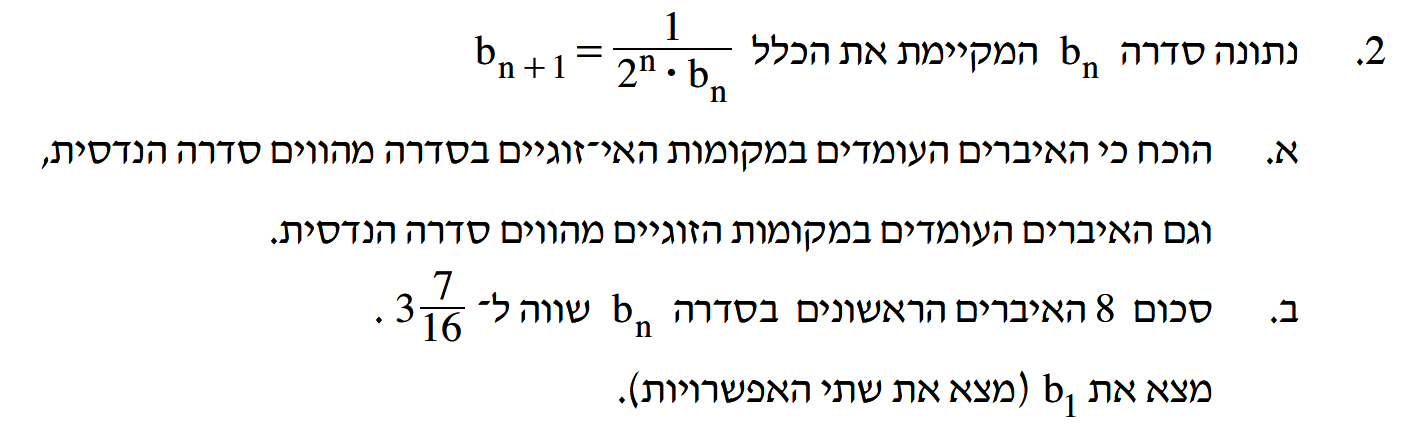
\includegraphics[width=.95\textwidth]{summer-2015b-2}
\end{center}
\vspace{-2ex}

\textbf{סעיף א}

החילוק של איברים במרחק שני מקומות אחד מהשני לא תלוי בזוגיות:
\[
\frac{b_{n+2}}{b_n} = \frac{1}{2^{n+1}\cdot b_{n+1}\cdot b_n}=\frac{1}{2^{n+1}\cdot\displaystyle\frac{1}{2^n\cdot b_n}\cdot {b_n}}= \frac{1}{2}\,.
\]
\textbf{סעיף ב}

אנחנו לא יודעים אם הסדרה כולה היא הנדסית, לכן נחשב בנפרד את הסכום 
של ארבעת האיברים הזוגיים וארבעת האיברים האי-זוגיים:
\erh{18pt}
\begin{equationarray*}{rcl}
S_{\mathit{odd}} &=& b_1+b_3+b_5+b_7=b_1\left(1 + \frac{1}{2} + \frac{1}{4} +\frac{1}{8}\right)=\frac{15}{8}b_1\\
S_{\mathit{even}} &=& b_2+b_4+b_6+b_8=b_2\left(1 + \frac{1}{2} + \frac{1}{4} +\frac{1}{8}\right)=\frac{15}{8}b_2=\frac{15}{8}\cdot\frac{1}{2^1b_1}\,.
\end{equationarray*}
מ:
\[
S_{\mathit{odd}} + S_{\mathit{even}} =\frac{15}{8}\left(b_1+\frac{1}{2b_1}\right)= 3\frac{7}{16}=\frac{55}{16}\,.
\]

נקבל משוואה ריבועית 
$6b_1^2-11b_1+3=0$
שיש לה שני פתרונות 
$\displaystyle b_1=\frac{3}{2},\,b_1=\frac{1}{3}$.

%%%%%%%%%%%%%%%%%%%%%%%%%%%%%%%%%%%%%%%%%%%%%%%%%%%%%%%%%%%%%%%%%%%
\np
\section{קיץ תשע"ה מועד א}

\begin{center}
\selectlanguage{english}
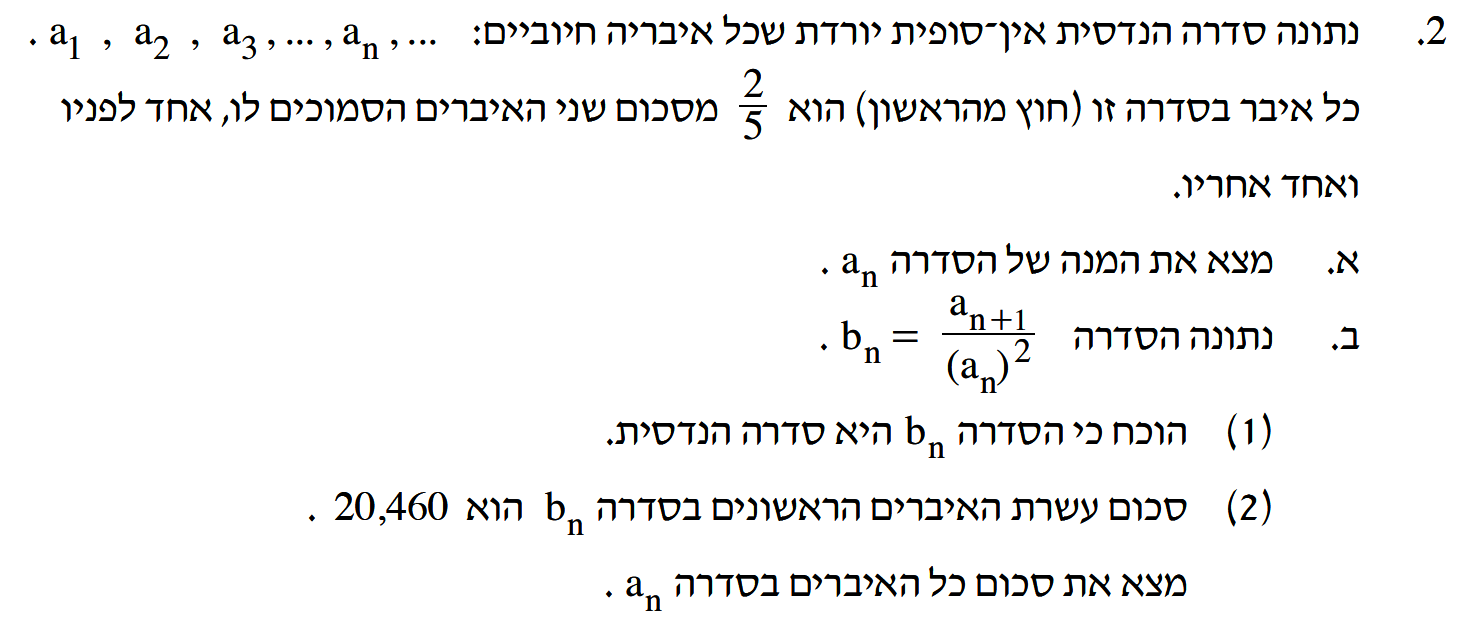
\includegraphics[width=.95\textwidth]{summer-2015a-2}
\end{center}
\vspace{-2ex}

\textbf{סעיף א}

נתון:
\[
a_n = \frac{2}{5}(a_{n-1}+a_{n+1}) =\frac{2}{5}\left(\frac{a_n}{q}+qa_n\right)
\]
עבור
$n\geq 2$.
$a_n$
מצטמצם ונקבל משוואה ריבועית
$2q^2-5q+2=0$
שיש לה שני פתורונות
$\displaystyle q=\frac{1}{2},	q=2$.
נתון שהסדרה יורדת ולכן
$\displaystyle q_a=\frac{1}{2}$.

\medskip

\textbf{סעיף ב}
$(1)$
\[
q_b=\frac{b_{n+1}}{b_n} = \frac{\displaystyle\frac{a_{n+2}}{(a_{n+1})^2}}{\displaystyle\frac{(a_{n})^2}{a_{n+1}}}= \frac{a_{n+2}}{(a_{n+1})^2}\cdot\frac{(a_{n})^2}{a_{n+1}} = \frac{a_nq^2}{(a_nq)^2}\cdot\frac{(a_n)^2}{a_nq}=\frac{1}{q}=2\,.
\]
\textbf{סעיף ב}
$(2)$

מ:
\[
S_{10}=\frac{b_1(2^{10}-1)}{2-1}=20460
\]
מתקבל
$b_1=20$.
השאלה מבקשת את סכום 
\textbf{הסדרה המקורית}
$a_{n}$.
כבר חישבנו את המנה
$q_a$
וניתן לחשב את
$a_1$
מהנוסחה עבור 
$b_n$:
\erh{16pt}
\begin{equationarray*}{rcl}
b_1 &=& \frac{a_2}{a_1^2} = \frac{a_1q_a}{(a_1)^2} = \frac{1}{2a_1}\\
a_1&=&\frac{1}{2b_1}=\frac{1}{40}\\
S_a &=& \frac{a_1}{1-q_a}=\frac{1}{40\left(1-\displaystyle\frac{1}{2}\right)} = \frac{1}{20}\,.
\end{equationarray*}

%%%%%%%%%%%%%%%%%%%%%%%%%%%%%%%%%%%%%%%%%%%%%%%%%%%%%%%%%%%%%%%%%%%

\np
\section{חורף תשע"ה}

\begin{center}
\selectlanguage{english}
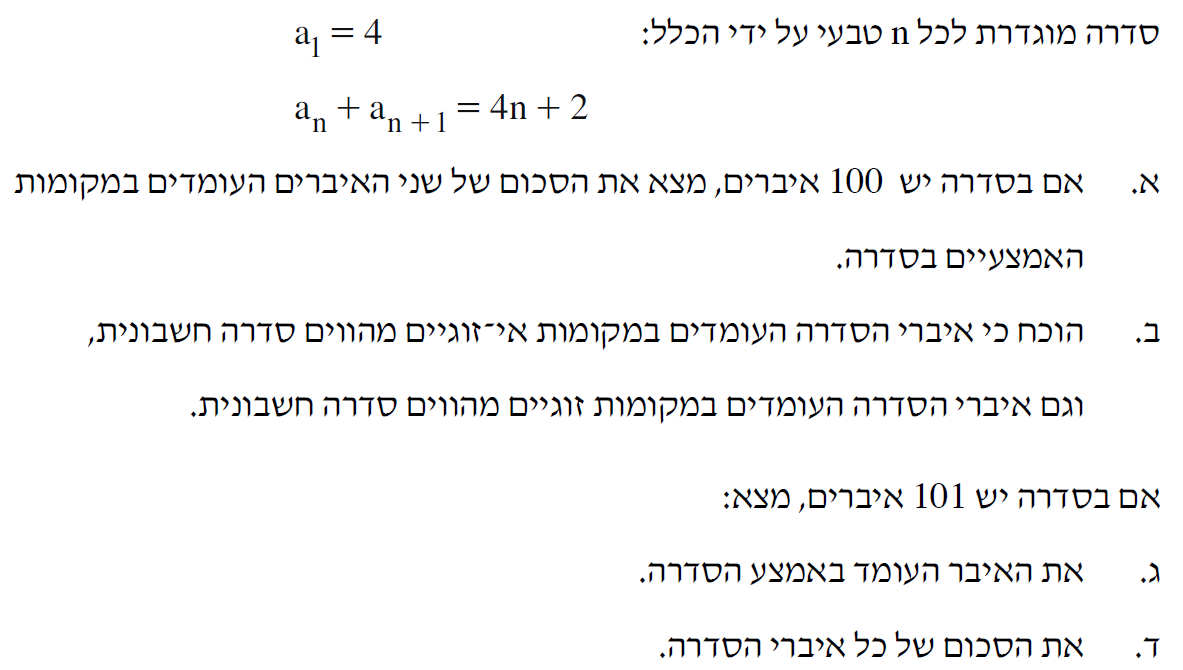
\includegraphics[width=.95\textwidth]{winter-2015-2}
\end{center}
\vspace{-1ex}

\textbf{שימו לב}
שלא נתון שהסדרה כולה היא חשבונית.

\textbf{סעיף א}

כדאי לרשום את איברי הסדרה כדי לוודא מהם האיברים האמצעיים:
\[
\overbrace{\rule{0pt}{8pt}a_1, a_2, \ldots, a_{49}, a_{50}}^{50}, \overbrace{\rule{0pt}{8pt}a_{51}, a_{52},\ldots, a_{100}}^{50}\,.
\]
ניתן לחשב את הסכום מהגדרת הסדרה:
\[
a_{50}+a_{51}=4\cdot 50+2=202\,.
\]
\textbf{סעיף ב}

במבט ראשון השאלה נראית בעייתית כי נתונה נוסחה לחישוב איברים סמוכים זה לזה
$a_n+a_{n+1}$,
אבל האיברים הזוגיים נמצאים במרחק שני מקומות זה מזה וכך גם האיברים האי-זוגיים
$a_{n+2}-a_{n}$.
חבל שאין לנו
$a_{n+1}-a_{n}$
ו-%
$a_{n+2}-a_{n+1}$.
צמד הביטויים האלה יכול לרמוז ל-"טריק" ידוע במתמטיקה: אם נוסיף ונחסיר את אותו ערך לביטוי, ערך הביטוי לא משתנה:
\begin{eqnarray*}
a_{k+2} - a_{k} &=& a_{k+2}+(a_{k+1}-a_{k+1})-a_{k}\\
&=& (a_{k+2}+a_{k+1})-(a_{k+1}+a_{k})\\
&=& (4(k+1)+2)-(4k+2)\\
&=&4\,.
\end{eqnarray*}
ההפרש קבוע ולא תלוי בזוגיות, ולכן הזוגיים והאי-זוגיים מהווים סדרות חשבוניות.

\np

\textbf{סעיף ג}

לא ידוע שהסדרה
$a_{n}$
חשבונית, אבל
$a_{51}$
הוא איבר בסדרת
\textbf{האי-זוגיים}.
נרשום את הסדרה כדי לדייק בספירת האיברים הזוגיים והאי-זוגיים:
\[
\overbrace{\rule{0pt}{8pt}a_1, a_2, \ldots, a_{49}, a_{50}}^{50}, a_{51}, \overbrace{\rule{0pt}{8pt}a_{52}, \ldots, a_{100}, a_{101}}^{50}\,.
\]
ברור שמספר האיברים האי-זוגיים גדול באחד ממספר האיברים הזוגיים,
$51$
אי-זוגיים ו-%
$50$
זוגיים. 
$a_{51}$
הוא האיבר ה-%
$25$
העומד באמצע הסדרה. האיבר הראשון של המספרים האי-זוגיים נתון,
$a_1=4$,
ואת ההפרש
$d=4$
חישבנו בסעיף הקודם. מכאן:
\[
a_{51}=a_1+25d =4+25\cdot 4=104\,.
\]

\textbf{סעיף ד}

נחשב את סכום הסדרה כחיבור של סכום האי-זוגיים וסכום הזוגיים.
$a_1=4$
נתון, וניתן לחשב לפי הנוסחה הנתונה:
\[
a_2=a_{1+1}=4\cdot 1+2-a_1=4+2-4=2\,.
\]
כבר חישבנו שהפרשים של שתי תת-הסדרות הם 
$4$.
מספר האי-זוגיים הוא
$51$
ומספר הזוגיים הוא
$50$.
הסכום הוא:
\[
S=S_{\mathit{odd}} + S_{\mathit{even}}=\frac{51}{2}(2\cdot 4+50\cdot 4)+\frac{50}{2}(2\cdot 2+49\cdot 4)=5304+5000=10304\,.
\]

%%%%%%%%%%%%%%%%%%%%%%%%%%%%%%%%%%%%%%%%%%%%%%%%%%%%%%%%%%%%%%%%%%%
\np

\section{קיץ תשע"ד מועד ב}

\begin{center}
\selectlanguage{english}
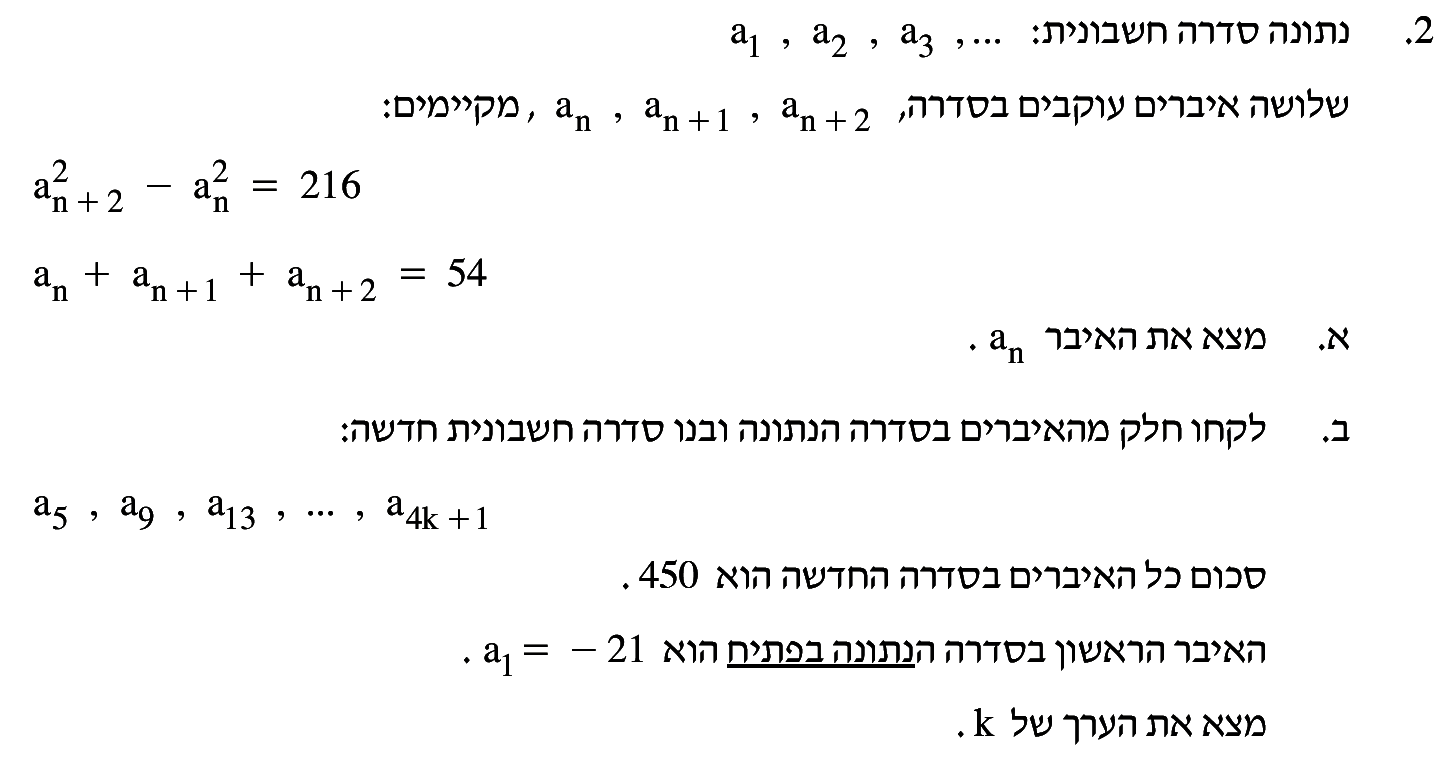
\includegraphics[width=.95\textwidth]{summer-2014b-2}
\end{center}
\vspace{-2ex}


\textbf{סעיף א}

הסדרה חשבונית ולכן ניתן להשתמש להציב בתוך המשוואות הנתונות ולקבל שתי משוואות עם שני נעלמים:
\erh{4pt}
\begin{equationarray*}{rcl}
(a_n+2d)^2 - a_n^2 &=& 216\\
4a_nd+4d^2 &=& 216\\
a_n+(a_n+d)+(a_n+2d)&=&54\\
3a_n + 3d &=& 54\,.
\end{equationarray*}
הפתרון הוא
$d=3,a_n=15$.

\smallskip

\textbf{סעיף ב}

הסדרה החדשה חשבונית שאיבריה 
$a'_1, a'_2,\ldots$
הם:
\[
\overbrace{a_5=a_1+4d}^{a_1'}, \quad a_6=a_5+5d,\quad  a_7=a_5+6d,\quad  a_8=a_5+7d,\quad  \overbrace{a_9=a_5+8d}^{a_2'}\,.
\]
בסדרה החדשה
$d' = 4d = 12$
ו-%
$a_1' = a_5 = -21 + 4d= -9$.
מסכום הסדרה החדשה:
\[
\frac{k}{2}(2a'_1 + (k-1)d')=\frac{k}{2}(-18+(k-1)\cdot 12)=450
\]
מתקבלת משוואה ריבועית
$2k^2-5k-150=0$
שהשורש החיובי שלה הוא
$k=10$.


%%%%%%%%%%%%%%%%%%%%%%%%%%%%%%%%%%%%%%%%%%%%%%%%%%%%%%%%%%%%%%%%%%%

\np
\section{קיץ תשע"ד מועד א}

\begin{center}
\selectlanguage{english}
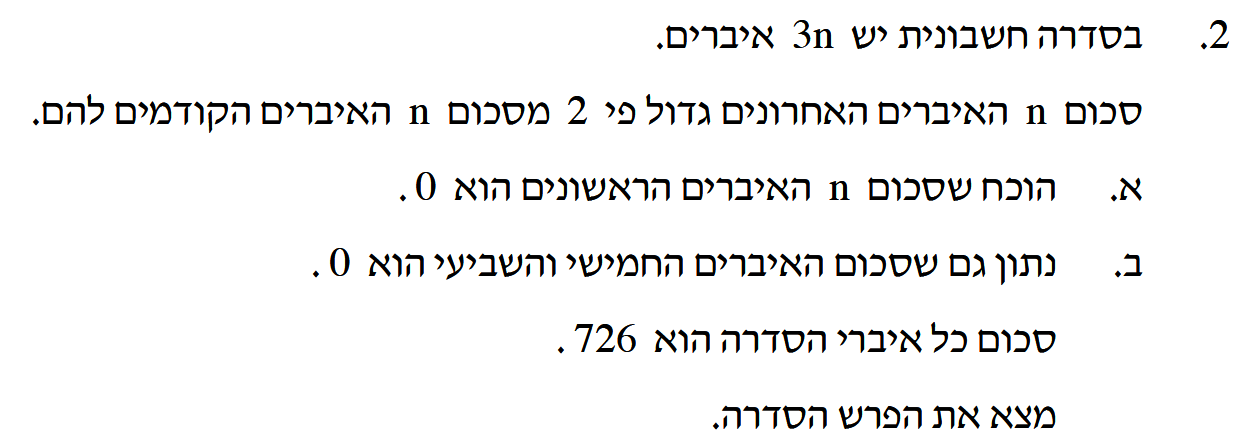
\includegraphics[width=.9\textwidth]{summer-2014a-2}
\end{center}

\vspace{-4ex}

\textbf{סעיף א}

כדי לדייק עם האינדקסים כדאי לרשום את הסדרה עם סימון של הסדרות החלקיות:
\[
\underbrace{
\overbrace{\rule{0pt}{8pt}a_1, a_2, \ldots, a_n}^{S_1},
\overbrace{\rule{0pt}{8pt}a_{n+1}, a_{n+2}, \ldots, a_{2n}}^{S_2},
\overbrace{\rule{0pt}{8pt}a_{2n+1}, a_{2n+2}, \ldots, a_{3n}}^{S_3}
}_{S_{3n}}\,.
\]
נתון
$S_3=2S_2$:
\[
\erh{10pt}
\begin{array}{lll}
\displaystyle\frac{n}{2}(2(a_1+2nd)+(n-1)d)&=&2\cdot \displaystyle\frac{n}{2}(2(a_1+nd)+(n-1)d)\\
2a_1+(5n-1)d&=&4a_1+(6n-2)d\\
2a_1+(n-1)d&=&0\,.
\end{array}
\]
הביטוי בצד השמאלי של המשוואה האחרונה הוא הסכום 
$S_1$.

דרך אחרת לפתור את הבעיה היא להחסיר את סכום התת-הסדרות מסכום הסדרה כולה:
\erh{14pt}
\begin{equationarray*}{rcl}
S_1&=& S_{3n} - (S_2+S_3) =  S_{3n} - (S_2 + 2S_2) = S_{3n} - 3S_2\\
&=&\displaystyle\frac{3n}{2}(2a_1+(3n-1)d) -3\cdot\displaystyle \frac{n}{2}(2(a_1+nd)+(n-1)d)\\
&=&0\,.
\end{equationarray*}

\np

\begin{center}
\fbox{
\begin{minipage}{.8\textwidth}
בבחינה של חורף תשע"ב אורך הסדרה הוא
$2n-1$,
ונתונים הסכומים של
$n$
האיברים הראשונים ו-%
$n$
האיברים האחרונים. רק רישום זהיר של הסדרה יבהיר שיש חפיפה בין שתי תת-הסדרות:
\[
\renewcommand{\arraystretch}{.3}
\begin{array}{ll}
\overbrace{\rule{0pt}{8pt}a_1, a_2, \ldots, a_n}^{n},&\hspace{-9pt}a_{n+1}, a_{n+2}, \ldots, a_{2n-1}\,.\\
&\hspace{-2em}\underbrace{\rule{10em}{0pt}}_{n}
\end{array}
\]
בדוגמה קל יותר לשים לב לחפיפה. עם
$n=4$:
\[
\renewcommand{\arraystretch}{.3}
\begin{array}{ll}
\overbrace{\rule{0pt}{8pt}a_1, a_2, a_3, a_4}^{4},&\hspace{-9pt}a_5, a_6, a_7\,.\\
&\hspace{-2em}\underbrace{\rule{5em}{0pt}}_{4}
\end{array}
\]
\vspace*{-1ex}
\end{minipage}
}
\end{center}

\bigskip

\textbf{סעיף ב}

נתון סכום הסדרה ועלינו למצוא
$d$
למרות שאין לנו 
$a_1$.
נבדוק אם הנתון השני יכול לעזור:
\[
a_5+a_7=(a_1 + 4d) + (a_1 + 6d) = 0\,.
\]
מכאן ש-%
$a_1=-5d$.


בסעיף א חישבנו ש-%
$S_1=0$
ונציב עבור 
$a_1$:
\[
\frac{n}{2}(-10d+(n-1)d)=0\,.
\]
$d$
לא יכול להיות
$0$
כי אחרת מהנתון שהסכום של שני איברים הוא אפס אפשר להסיק שכל איברי הסדרה הם אפס. זה סותר את הנתון שהסכום הוא מספר חיובי. לכן אפשר לחלק את המשוואה ב-%
$d$
ונקבל
$n=11$.

נציב עבור
$a_1,n$
בנוסחה ל-%
$S_{3n}$:
\erh{16pt}
\begin{equationarray*}{rcl}
S_3&=&\frac{3n}{2}(2a_1+(3n-1)d)\\
&=&\frac{33}{2}(-10d+(33-1)d)\\
&=&\frac{33}{2}\cdot 22d = 363d=726\,,
\end{equationarray*}
ונקבל 
$d=2$.

%%%%%%%%%%%%%%%%%%%%%%%%%%%%%%%%%%%%%%%%%%%%%%%%%%%%%%%%%%%%%%%%%%%
\np

\section{חורף תשע"ד}

\begin{center}
\selectlanguage{english}
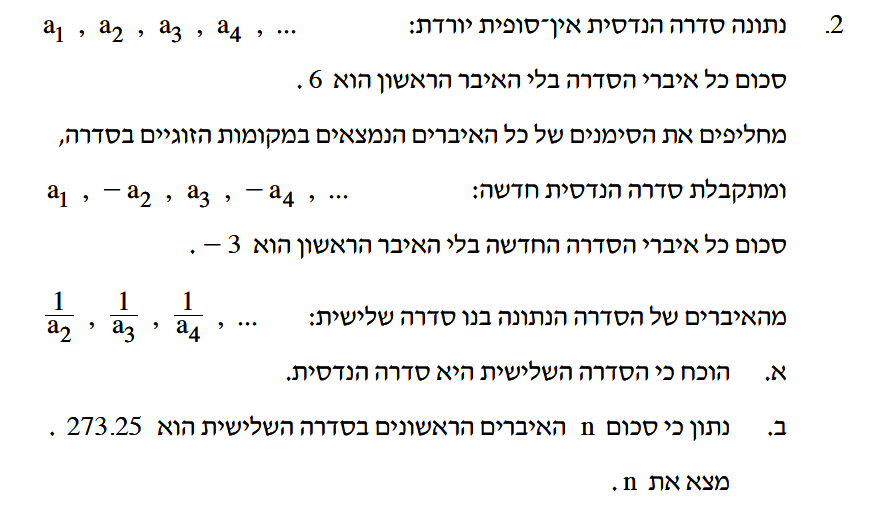
\includegraphics[width=.9\textwidth]{winter-2014-2}
\end{center}
\vspace{-2ex}
\textbf{סעיף א}

המנה של הסדרה השלישית קבועה כי נתון שהסדרה הראשונה הנדסית:
\[
\frac{1/a_{n+1}}{1/a_n}=\frac{a_n}{a_{n+1}}\,.
\]
\textbf{סעיף ב}

נשתמש בשני הסכומים הנתונים כדי לכתוב שתי משוואות עם שני נעלמים:
\erh{12pt}
\begin{equationarray*}{rcl}
\frac{a_2}{1-q}&=&6\\
\frac{-a_2}{1-(-q)}&=& -3\,.
\end{equationarray*}
הפתרון הוא 
$q=\displaystyle\frac{1}{3}$
ו-%
$a_2=4$.

בסדרה השלישית, האיבר הראשון הוא 
$\displaystyle \frac{1}{a_2}=\frac{1}{4}$
וההפרש הוא
$\displaystyle \frac{1}{d}=3$
מהסכום השלישי ונקבל:
\erh{12pt}
\begin{equationarray*}{rcl}
\frac{1}{4}\cdot \frac{3^n-1}{3-1}&=&273.25\\
3^n&=&2187\\
n&=&7\,,
\end{equationarray*}
כאשר בדקנו חזקות של
$3$
עד שהתקבל
$2187$.



%%%%%%%%%%%%%%%%%%%%%%%%%%%%%%%%%%%%%%%%%%%%%%%%%%%%%%%%%%%%%%%%%%%

\selectlanguage{english}
\clearpage
\selectlanguage{hebrew}

\section*{המלצות}

\addcontentsline{cot}{chapter}{המלצות: סדרות}


\begin{itemize}


\item
\textbf{חובה לקרוא את השאלות בזהירות רבה.}
בבחינה של קיץ תשע"ה א, סעיף ב שואלת על סדרה חדשה
${b_n}$
אבל בסוף חוזרת ומבקשת למצוא את הסכום של הסדרה הנתונה
${a_n}$.

\item
שימו לב אם סדרה היא חשבונית, הנדסית או לא זו ולא זו.

\item 
ברוב השאלות נתונה סדרה ומוגדרת סדרה חדשה המובססת על הסדרה הנתונה. 
\textbf{אין בהכרח קשר}
בין תכונה של הסדרה המקורית והסדרה החדשה. להלן שתי סדרות חשבוניות, אבל כאשר משלבים את שתיהן, מתקבלת סדרה שאיננה חשבונית:
\[
\begin{array}{rrrrrrrrrrr}
1,& 4,& 7,& 10,& 13,& \ldots\\
2,& 5,& 8,& 11,& 14, &\ldots\\
1,& 2,& 4,& 5,& 7,& 8,& 10,& 11,& 13,& 14, &\ldots
\end{array}
\]
\item
כאשר מבקשים להוכיח שתת-סדרת הזוגיים חשבונית או הנדסית וגם תת-סדרת האי-זוגיים, הוכחה אחת תספיק כי אם 
$\displaystyle \frac{a_{n+2}}{a_n}$
קבוע, לא משנה אם 
$n$
זוגי או אי-זוגי.


\item
כדאי לרשום את איברי הסדרה כדי לדייק במקומות של האיברים:
\[
\setlength{\extrarowheight}{8pt}
\begin{array}{l}
\overbrace{\rule{0pt}{8pt}a_1, a_2, \ldots, a_{49}, a_{50}}^{50}, \overbrace{\rule{0pt}{8pt}a_{51}, a_{52},\ldots, a_{100}}^{50}\\
\underbrace{\rule{0pt}{8pt}a_1, a_2, \ldots, a_{49}, a_{50}}_{50}, a_{51}, \underbrace{\rule{0pt}{8pt}a_{52}, \ldots, a_{100}, a_{101}}_{50}\,.
\end{array}
\]
\vspace{-3ex}

\item
מקרה מעניין הוא תת-סדרות חופפות )בחינה של חורף תשע"ב שלא נמצאת במסמך זה(:
\[
\renewcommand{\arraystretch}{.4}
\begin{array}{ll}
\overbrace{\rule{0pt}{8pt}a_1, a_2, \ldots, a_n}^{n},&\hspace{-9pt}a_{n+1}, a_{n+2}, \ldots, a_{2n-1}\\
&\hspace{-2em}\underbrace{\rule{10em}{0pt}}_{n}
\end{array}
\]
\vspace{-4ex}
\item
קיימות שתי דרכים לסכם מספר תת-סדרות )בחינה של קיץ תשע"ד א(. דרך אחת היא לסכם כל תת-סדרות בנפרד עם ערכי ה-%
$d, a_1$
או
$n, q$
שלהן. זה קורה לעתים קרובות כאשר השאלה מבקשת לחשב סכום של סדרה, אבל ידוע רק שתת-סדרות חשבוניות או הנדסיות, למשל, זוגיים ואי-זוגיים )בחינה של קיץ תשע"ח ב(.
\item 
דרך אחרת היא לחבר הסכומים של תת-סדרות ולהחסיר את התוצאה מסכום הסדרה כולה:
\[
S_1 = S_n - (S_2+S_3)\,.
\]
\vspace{-6ex}

\item
בסדרה קיימים ארבעה נעלמים
$d, a_1$
או
$S, n, q$.
כדי למצוא את ערכו של נעלם אחד, צריך לדעת את ערכי שלושת הנעלמים האחרים )או שניים אם לא מדובר בסכום(. לפעמים, מספיק לדעת את הקשר בין שני נעלמים, כגון
$a_1+11d = 0$
בבחינה של הורף תשע"ח.

\np

\item
הבחינה של חורף תשע"ו מעניינת כי מספר האיברים הוא לא הערך של המספר 
$n$
המופיע בשאלה. חשוב לרשום דוגמה מספרית כדי לוודא מהו מספר האיברים:
\[
(1)\, a_1\cdot a_2,\;\; (2)\,a_2\cdot a_3,\;\;\cdots\;\; (5)\,a_5\cdot a_6=(a_n\cdot a_{n+1}),\;\; (6)\,a_6\cdot a_7 \;(= a_{n+1}\cdot a_{n+2})\,.
\]
\vspace{-4ex}

\item
טריק שימושי הוא לחבר ולהחסיר את אותו ערך בביטוי )בחינה  חורף תשע"ה(:
\[
a_{k+2} - a_{k} = a_{k+2}+(a_{k+1}-a_{k+1})-a_{k} = (a_{k+2}+a_{k+1})-(a_{k+1}+a_{k})\,.
\]
\vspace{-4ex}

\item
הכנסת איברים חדשים בתוך סדרה לא בהכרח שומרת על הסדרה כחשבונית או הנדסית. השורה הראשונה להלן היא סדרה חשבונית. בשורה השנייה הוכנסו איברים של סדרה חשבונית נוספת והסדרה החדשה היא חשבונית. בשורה השלישית הוכנסו איברים של סדרה חשבונית נוספת והסדרה החדשה איננה חשבונית.
\[
\begin{array}{rrrrrrrrrrrrr}
1,& 5,& 9,& 13,& 17\\
1, &3,& 5,&7,& 9,& 11,& 13, &15, & 17\\
1, &2,& 5,&6,& 9,& 10,& 13, &14, & 17
\end{array}
\]
בבחינה של קיץ תשע"ו ב כתוב במפורש שהסדרה חדשה חשבונית.

\item
בhישוב הפרש או מנה, כדאי להציב ב-%
$a_{n+1}$
או
$a_{n-1}$
ביטוי שיש בו 
$a_n$.
הנה דוגמה מהבחינה של  קיץ תשע"ה א:
\[
a_n = \frac{2}{5}(a_{n-1}+a_{n+1}) =\frac{2}{5}\left(\frac{a_n}{q}+qa_n\right)\,.
\]
$a_n$
מצטמצם ונקבל משוואה ריבועית ב-%
$q$.

\end{itemize}

\selectlanguage{english}
